To overcome the above challenges, we propose a two-phase MapReduce framework, as shown in Figure~\ref{figure:framework}. In the first phase(See Section~\ref{firstPhase}), instances of objects are evenly mapped to $N$ machines through angle-based partition scheme, and unqualified objects are filtered out based on Rectangle pruning rules, as these unqualified objects are not able to be in the $p-$skyline object set. Objects which are not filtered in this phase become candidate objects and are outputted in the reduce function. In the second phase(See Section~\ref{secondPhase}), all candidate objects are grouped into several machines based on a novel grid partition, and object skyline probability is computed locally in separate machine. After that, $p-$skyline object set is easily obtained.
\begin{figure*}[t]
\centering
  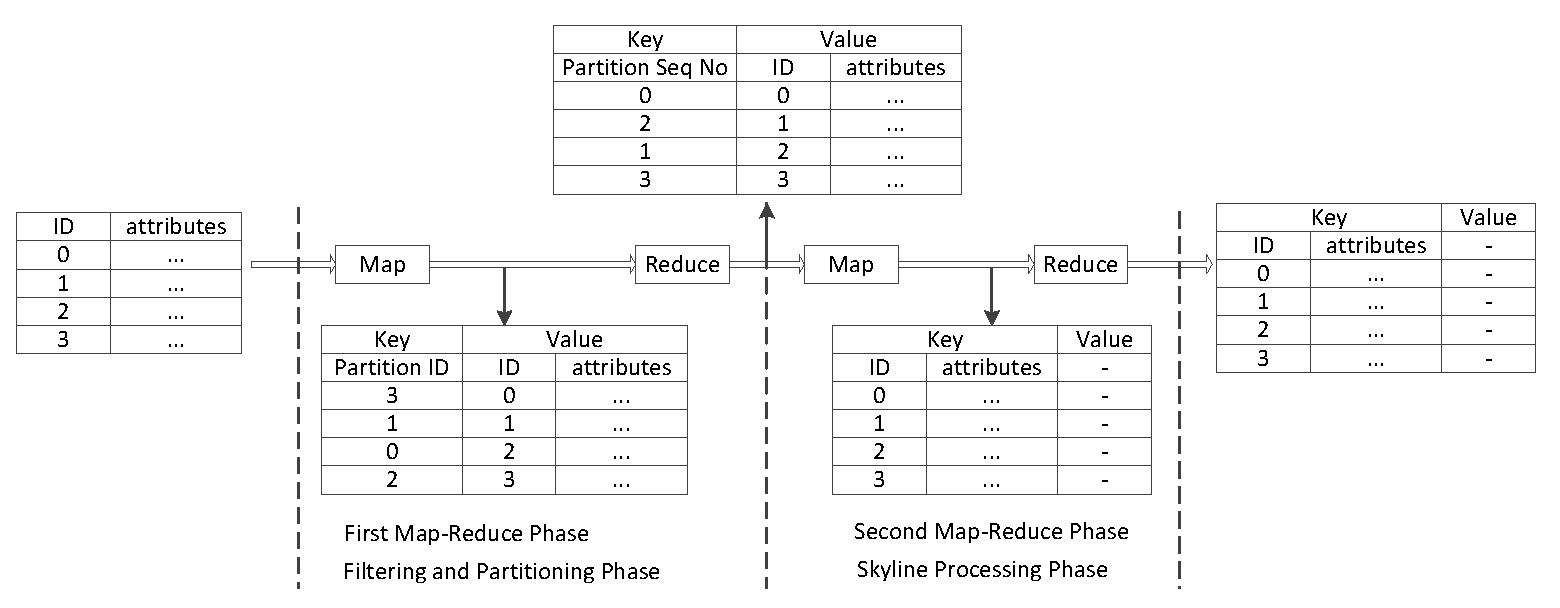
\includegraphics[width=0.9\textwidth]{figs/framework.eps}
  \vspace*{-10pt}
  \caption{An overview of parallel skyline processing using MapReduce.}
  \vspace*{-15pt}
  \label{figure:framework}
\end{figure*}

\subsection{Partitioning}

Angle-based space partitioning scheme~\cite{ref:AngularPartition} transforms data point from Cartesian coordinate to hyperspherical coordinate. In the first map phase, we use angle-based partitioning strategy to map data points into N partitions. The main advantage of angular transformation is that this strategy being able to filter data points as much as it can since the left bottom corner data points dominate most other data points in an angle.

Given a d-dimensional data point $p = [p_1, p_2, \dots, p_d]$, the hyperspherical coordinates of $p$ include a radial coordinate $r$ and $d-1$ angular coordinates $\varphi_1, \varphi_2, \dots, \varphi_{d-1}$~\cite{ref:AngularPartition}, denoted by $\{r, \varphi_1, \varphi_2, \dots, \varphi_{d-1}\}$, where r is the distance to the origin, and $\varphi_i$ represents an angular coordinate $ 0 \leq  \varphi_i \leq \frac{\pi}{2}$. Similarly, an angle-based space partition is represented by $V^A = \{\Phi_1^A, \Phi_2^A, \dots, \Phi_{d-1}^A \}$, where $\Phi_i^A$ is an angle range $[\varphi_i^j,\varphi_i^k]$ in the $i^{th}$ dimension.

In term with the detailed implementation of the Map Phase, the number of reducers have been defined prior to the launch of the application, and the default partitioning angles $V^A$ has been computed. The whole instance dataset is an input to Map function. 

% In the Map phase, angular coordinates of data point of every instance are computed, and mapped to target reducer.

\subsection{Pruning Power}
Given an object $O = \{p_1, p_2, \dots, p_m\}$, the minimum corner of one object $O_{min}$, is represented by a $d-$dimensional virtual point $( \min\limits_{p_i \in O}p_i[1], \min\limits_{p_i \in O}p_i[2], \dots, \min\limits_{p_i \in O}p_i[d])$, where $p_i$ is an instance in $O$. Similarly, $O_{max}$ is a maximum corner point.

\vspace{5 mm}
\begin{lemma}
\label{lemma:1}
Given $O^a, O^b \in O$, \emph{if} $O^a_{max} \prec O^b_{min}$, then $SKYProb(O^b) = 0$, $O^b \notin PSKY(OS)$.
\end{lemma}

\vspace{5 mm}

\begin{lemma}
\label{lemma:2}
Given $O^a \in O$, an instance $p \notin O^a$, \emph{if} $O^a_{max} \prec p$, $SKYProb(p) = 0$.
\end{lemma}

\vspace{5 mm}

The proof of Lemma~\ref{lemma:1} and Lemma~\ref{lemma:2} is obvious and omitted.
Besides, we compute the probability of one object $O_a$ being a skyline object with partially seen data. And the upper bound of it is denoted by $SKYProb^{+}(O)$. Similarly, $SKYProb^{+}(p)$ represents the probability of an instance $p$ being a skyline instance.

\vspace{5 mm}

\begin{lemma}
\label{lemma:3}
Given $O^a \in O$, $O^a=\{p_1, p_2, \dots, p_m\}$, $|O^a| = m$, $O^a$'s instances are mapped into several partitions (machines). Assume partition $V^A$ has $n$ instances out of $m$ ($n<=m$) for $O_a$, containing instances $\{p_1, p_2, \dots, p_n\}$. Then:

\begin{equation}
\label{objectUpper}
    \begin{aligned}
PrSKY^{+}(O_a) = 1 - \sum\limits_{i=1}^n Pr(p_i)(SKYProb^+(p_i)-1)
    \end{aligned}
\end{equation}

\emph{if} $SKYProb^{+}(O_a) < p$, then $O_a \notin PSKY(OS)$.

\end{lemma}

\begin{proof}
The Skyline Probability of an object $O_a$ is denoted as:
\begin{equation}
    \begin{aligned}
SKYProb(O_a) = \sum\limits_{i=1}^n Pr(p_i)(SKYProb(p_i))
    \end{aligned}
\end{equation}

\begin{equation}
    \begin{aligned}
\sum\limits_{i=1}^n Pr(p_i) = 1
    \end{aligned}
\end{equation}

Then, 
\begin{equation}
    \begin{aligned}
& SKYProb^{+}(O_a) \\
& <= \sum\limits_{i=1}^n Pr(p_i)(SKYProb(p_i)) +
\sum\limits_{i=n+1}^m Pr(p_i) \\
& <= \sum\limits_{i=1}^n Pr(p_i)(SKYProb^+(p_i)) +
1 - \sum\limits_{i=1}^n Pr(p_i) \\
& = 1 - \sum\limits_{i=1}^n Pr(p_i)(SKYProb^+(p_i)-1)
    \end{aligned}
\end{equation}
\end{proof}


\subsection{First Phase}
\label{firstPhase}
Before the first phase MapReduce job is launched, every object $O$'s $O_{min}$ and $O_{max}$ is computed locally by iterating all objects and computing $O_{min}$ and $O_{max}$ of every object.

The first map phase maps data points (instances) to $N$ machines based on angular partition scheme. The defined map function computes every instance's hyperspherical coordinate, and maps instances to designated reducer (machine). In addition, if any instance of one object $O$ is mapped to a reducer $V^A$, maximum and minimum corner of $O$ ($O_{min}$ and $O_{max}$) is also transmitted to the partition. Therefore, $O_{min}$ and $O_{max}$ of one object might appear in more than one partitions, since instances of one object are distributed in more than one partitions.

During the reduce phase, only data in this partition (data in $V^A$) is visible. Objects are firstly examined if some of them is able to be pruned under the Pruning rule 1. The procedure to examine Pruning rule 1 works as follows. A list $L_{min}$ contains all $O_{min}$ of all objects in this partition; similarly, a list $L_{max}$ contains all $O_{max}$ in this partition. Sort-filter-skyline~\cite{icde/ChomickiGGL03} method is an approach to speed up traditional skyline query by presorting instances. Using $SFS$, data points with the sum of all the dimensions of each point is presorted in ascending. The starting element is retrieved from $L_{max}$, and compared with the elements in $L_{min}$ to check the dominance relationship. Any object whose $O_{min}$ is dominated by any $O_{max}$ in $L_{max}$ is pruned, since it can not be in the $p-$skyline set.

After this, Pruning rule 2 works as follows. In every reducer, we collected remained objects which are not pruned in $L_{min}$. For every instance in these remained objects, we check if an instance $p$ is dominated by some objects's $O_{max}$. If the dominance relationship occurs ($O_{max} \prec p$), $SKYProb(p)$ is marked to $0$ for the instance and it denotes that $p$ can not become skyline instance.

\subsection{Rectangle Pruning}
\label{secondPhase}
In this subsection, we propose a novel strategy to apply Lemma~\ref{lemma:3} to filter unqualified objects in partition $V^A$. As we see in Equation~\ref{objectUpper}, before $SKYProb^{+}(O_a)$ is computed, every instance's $SKYProb^{+}(p)$ contained in this partition is computed. Therefore, the challenge comes from how to efficiently collect the probability of every instance $p$ being a skyline instance.
The straightforward method of computing $SKYProb^{+}(p)$ is to iterate every instance in this partition, and compare the dominance relationship between $p$ and every other local instances in this partition. The computing complexity is obviously high as $O(n^2)$.

\begin{figure}[t]
\vspace{-15pt}
\centering
  \centerline{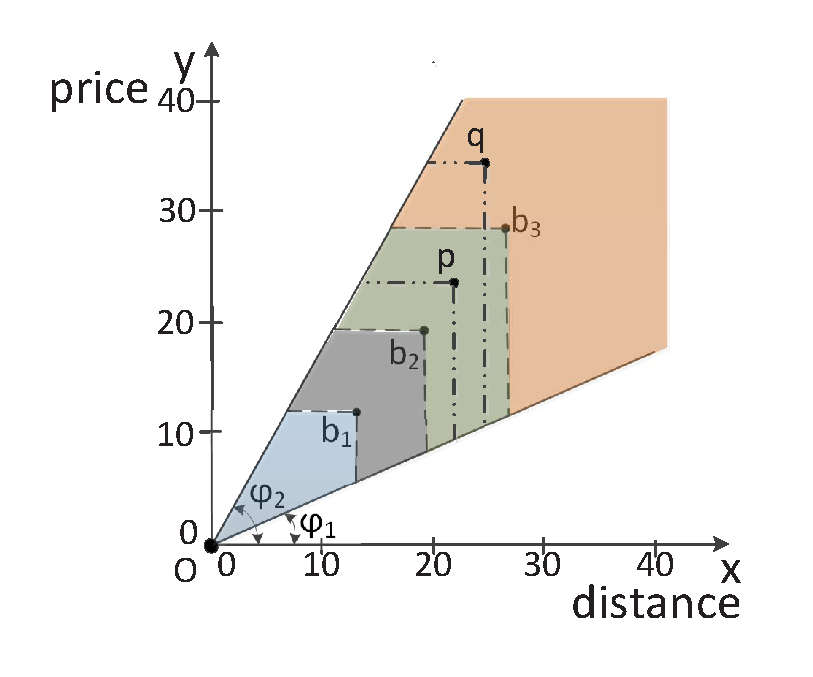
\psfig{file=figs/rectExample.eps,width=4.0in}}
  \caption{Prune 3}
  \vspace{-15pt}
  \label{figure:rect}
\end{figure}

One interesting observation is that data points close to maximum boundary are often dominated by data points close to minimum boundary. The intuitive idea is to associate data points close together into a group. Pre-computing is done in the group before probabilistic skyline process is launched. Data points fully dominated by the group is able to speed up processing by repeatedly applying the pre-computed information.

Take 2-dimensional data as an example (See Figure~\ref{figure:rect}). Assume the angle of partition $V^A$ is between $\phi_1$ and $\phi_2$. Three virtual data points $b_1$, $b_2$ and $b_3$ separate $V^A$ into four areas, denoted by 4 colors, blue, grey, green and red in order. Every point stands at the maximum corner of a bounding box. $p$ is an instance located in green area. It is observed that $p$ is always dominated by any instance in blue and grey areas since $b_2$ dominates $p$, and $p$ is also affected by partial instances in green area. Similarly, all instances in blue and grey areas and partial instances in green and red areas dominate $q$. According to this observation, we are able to precompute the sum of existing instance probabilities in blue and grey areas, and use the intermediate result for computing $SKYProb^{+}(p)$ and $SKYProb^{+}(q)$. Obviously it is able to speed up the skyline probability computing. 

We use pivot point set $P$ to represent the virtual data points (in Figure~\ref{figure:rect}), defined as a set of d-dimensional data points whose cardinality is m, $P=\{b_1, b_2, \dots, b_m\}$. $A_i$ is denoted as the d-dimensional hyper-rectangle, the minimum corner of which is the origin, and the maximum corner of which is $b_i$. If some point is dominated by $b_i$, it is dominated by any instance in $A_i$. Formally let each area $A_i$ consists of an n-dimensional vector $V_i = [p_{r1}, p_{r2}, \dots, p_{rn}]$, where $n$ is the number of objects in this partition (reducer), and each element $p_{ri}$ is the sum of instance probability for object $O_i$. These vectors is able to repeatedly contribute to the skyline probability of data points.  


\begin{figure}[t]
\vspace{-15pt}
\centering
  \centerline{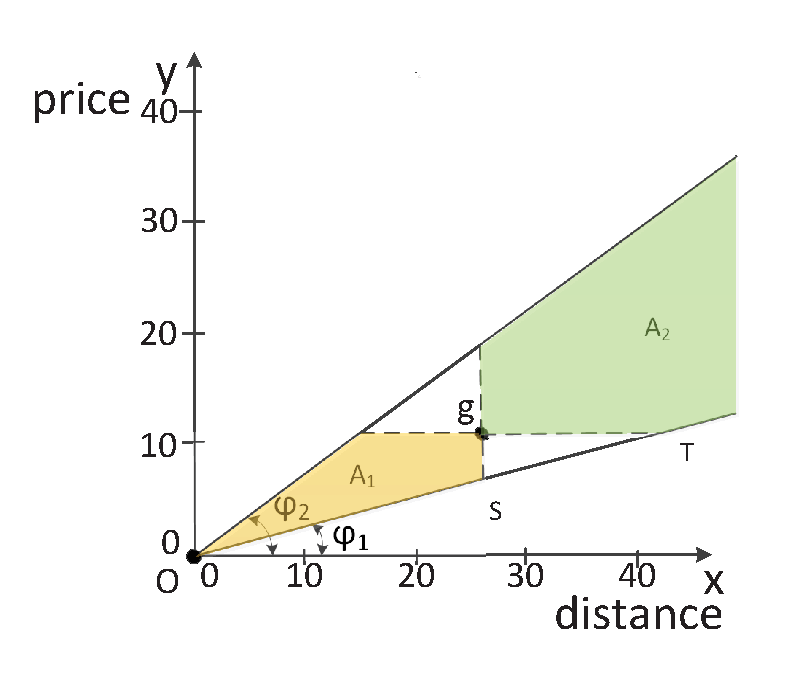
\psfig{file=figs/computeA_1.eps, width=4.0in}}
  \caption{Pruning Power}
  \vspace{-15pt}
  \label{figure:A1A2}
\end{figure}

Now the problem turns to studying the pruning power of a pivot point $g$. We make the assumption that our dataset is defined in the hypercube $[0,1]^d$ and data points are uniformly distributed. Followed by this assumption, the number of data points located in a region could be represented by the region's volume. To simplify the model of pruning power, only one pivot point exists and it divides the angle area into two parts denoted as $A_1$ and $A_2$. $A_1$ lies in the left bottom to g, and $A_2$ lies in the right top to g. Figure~\ref{figure:A1A2} depicts the scenario. The pruning power could be represented by how many data points in $A_2$ is able to repeatedly use $A_1$ directly without comparing one by one, since intermediate sum of instance probability in $A_1$ has been computed well. Therefore, given a pivot point $g$, the pruning power of $g$ is defined as:

\begin{equation}
PP(g) = A_1(x_g, y_g, \phi_1, \phi_2) * A_2(x_g, y_g, \phi_1, \phi_2)
\end{equation}
where $A_1$ or $A_2$ is a function, which computes corresponding area shown in Figure~\ref{figure:A1A2}.

In~\cite{ref:AngularPartition}, how to compute $A_2$ is introduced. Three cases are considered in formula induction: one is $0 \leq \phi_1 < \phi_2 \leq \pi/4$, the other is $\pi/4 \leq \phi_1 < \phi_2 \leq \pi/2$, and the final one is $0 \leq \phi_1 \leq \pi/4 \le \phi_2 \leq \pi/2$. The detailed formula is shown in Equation~\ref{Equ:A2}.

\begin{equation}
\label{Equ:A2}
A_2 = 
\begin{cases}
& \int_{x_g}^{1} \int_{x tan \phi_1}^{x tan \phi_2} dydx- \int_{x_g}^{min(1, \frac{y_g}{tan \phi_1})} \int_{x tan \phi_1}^{y_g} dydx  \\
& \qquad \qquad \qquad \qquad \mbox{if } 0 \leq \phi_1 < \phi_2 \leq \pi/4 \\ 
& A_2(g_y, g_x, \frac{\pi}{2} - \phi_2, \frac{\pi}{2} - \phi_1)\\
& \qquad \qquad \qquad \qquad \mbox{if } \pi/4 \leq \phi_1 < \phi_2 \leq \pi/2 \\
& A_2(x_g, y_g, \phi_1, \frac{\pi}{4}) + A_2(g_y, g_x, \frac{\pi}{2} - \phi_2, \frac{\pi}{4}) \\
& \qquad \qquad \qquad \qquad \mbox{if } 0 \leq \phi_1 \leq \pi/4 \le \phi_2 \leq \pi/2
\end{cases}
\end{equation}

Similarly, we compute the area of $A_1$, which is the region defined by $0 \le x \le x_g$, and $x tan(\phi_1) \le y \le min(x tan(\phi_2), y_g)$. Therefore, $A_1$ is represented by 

\begin{equation}
A_1 = \int_{0}^{x_g} \int_{x tan(\phi_1)}^{ min(x tan(\phi_2), y_g) } dydx
\end{equation}


Assume that $0 \leq \phi_1 < \phi_2 \leq \pi/4$, $PP(g)$ is represented by 
\begin{equation}
\begin{aligned}
PP(g) = & (\int_{x_g}^{1} \int_{x tan \phi_1}^{x tan \phi_2} dydx- \int_{x_g}^{min(1, \frac{y_g}{tan \phi_1})} \int_{x tan \phi_1}^{y_g} dydx)  \\
  & * \int_{0}^{x_g} \int_{x tan(\phi_1)}^{ min(x tan(\phi_2), y_g) } dydx
\end{aligned}
\end{equation}

It is found that the pruning power is dependent on the cardinality of $P$ and the placement of $P$ in the partition. Given the formula of pruning power computation, the set of pivot points is studied via experiment. We assume the 2-dimensional space is partitioned into 4 partitions. In each angle partition, the same experiment is executed.


We firstly study the relationship between the number of pivot points and the pruning power. We iteratively sample N points, from 1 to 100. For every iteration, pivot points are sampled 10,000 times. We obtain the pruning power of every iteration based on the sum of all 10,000 samples' pruning power value. For example, when $N=3$, three nodes are uniformly sampled in one partition. the sum of pruning powers of the three points is repeated 10,000 times and the addition of all is the final result. The experiment results shows that the pruning power increases with the elevation of the number of pivot points. Secondly, the distribution of pivot points is studied. We assume that only 1 pivot point is put in the partition. After sampling 10,000 times, we are looking for the location of pivot point, which has the most pruning power. The experiment shows that the points in the middle area have the most pruning power.  

Given the number of pivot points, we propose an efficient strategy to utilize the pruning power of pivot points. Pivot points in $P$ are selected every even interval of x, and lied in a line $L$ at an angle of $\phi_3$ ($ \phi_2 < \phi_3 < \phi_1 $) (See Figure~\ref{figure:midLine}).

% For each sample with an $x_g$, we obtain three pivot point candidates. Then each pivot point candidate ($x_g$, $y_g$) is obtained by $y_g = x_g * tan(\phi_g)$, where $\phi_g$ is predefined. Figure~\ref{figure:midLine} shows the cases when three pivot point candidates stand in three positions when the angle changes. The three points are located in lines at angle of $\phi_1$, $\phi_2$, and an angle between $\phi_1$ and $\phi_2$. The pivot points are selected when $x$ value varies from 0.1 to 0.9. Figure~\ref{figure:testArea} depicts the experiment result. From the smallest x value to the largest, pivot point candidates upon top line always outperform than other two lines. It is also found that points in the center area ($0.5 \leq x_g \leq 0.8$) have more pruning power.


\begin{figure}[!b]
\vspace{-15pt}
\centering
  \centerline{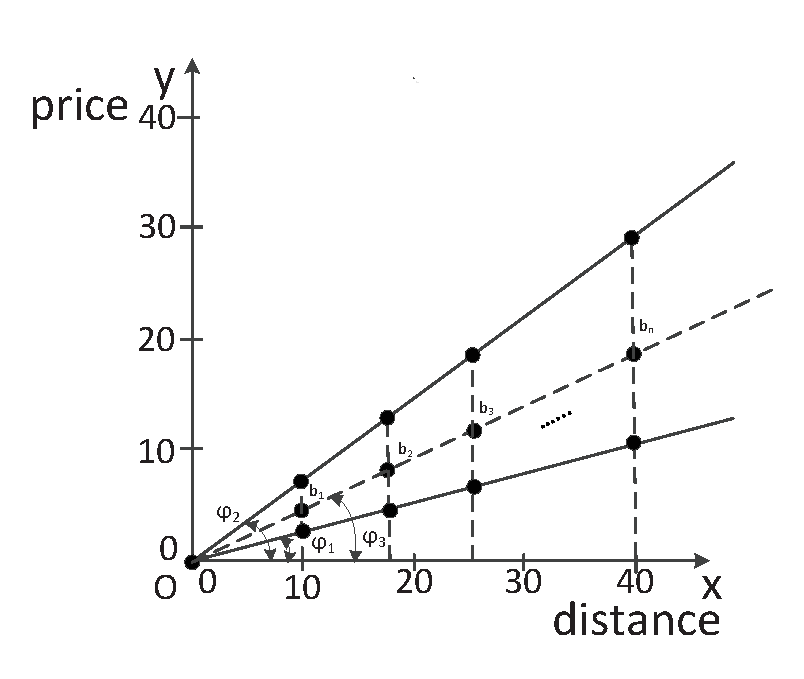
\psfig{file=figs/midLine.eps, width=3.5in}}
  \caption{Pivot Points placement}
  \vspace{-15pt}
  \label{figure:midLine}
\end{figure}

\begin{figure}[t]
\vspace{-15pt}
\centering
  \centerline{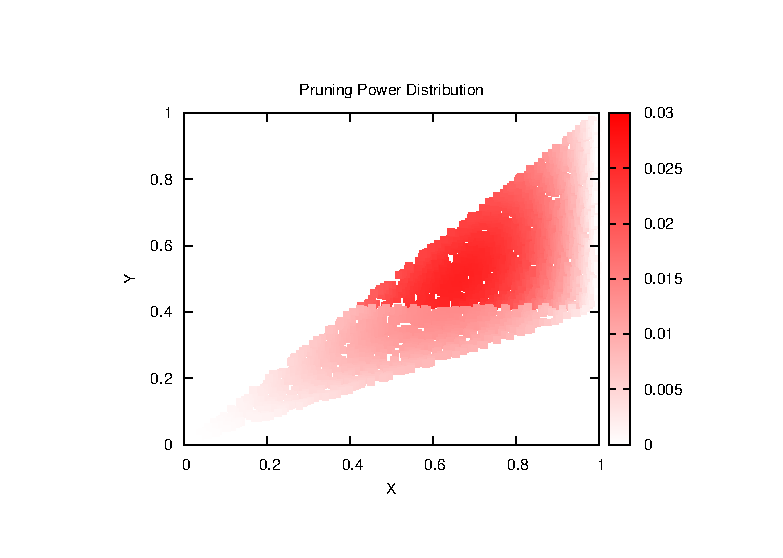
\psfig{file=Exper/MostPruningPower/3d.eps, width=3.5in}}
  \caption{line}
  \vspace{-15pt}
  \label{figure:testArea}
\end{figure}

% Based on the experiment result, in order to maximize the pruning power of pivot point, we let pivot points lie in a line $L$ at an angle of $\phi_2$. Given an input number $N_p$ of how many pivot points are put, 


Given pivot point set $P$ is placed well, the detailed computing procedure is as follows. Remember $A_i$ consists of an n-dimensional vector $V_i = [p_{r1},p_{r2},\dots,p_{rn}]$, where n is the number of objects in this partition. $V_i$ is maintained in the first step. At the beginning of the reduce phase, the local machine knows which objects are in this partition. Given an instance $p$ of object $O_q$, we firstly search the nearest pivot point $b_i$ dominated by $p$. Then the instance probability is added to $p_{rq}$ in $V_i$. We iterate every instance in the partition and maintain $V_i$ ($ 1 \leq i \leq n$). 

After $V_i$ is finished maintaining, every instance $p$ is iterated for computing $SkyProb^+(p)$. Assume an instance $p$ lies in the area $A_m$. we looks for the nearest $b_i$ which dominates $p$. $A_i$ fully dominates $p$. In addition, we look for area set $S_A$ which partially dominates $p$. $S_A$ = $\{A_j| i < j \leq m \}$.
An additional vector $[p_{r1},p_{r2},\dots,p_{rn}]$ is maintained for comparing domination relationship in $S_A$. If any instance in $S_A$ dominate $p$, the instance's existing probability is counted to the object vector. Then, aggregated by the vectors $V_j$ ($j \leq i$) precomputed already, the product of every element in the object vector is the final $SkyProb^+(p)$.

Then skyline likelihood of every object in $V^A$ is able to be easily obtained by Equation~\ref{objectUpper}. We could prune those unqualified objects with $SKYProb(O)$ less than $p$, and keep remained ones in an object set $C_o$.

\begin{defn}
\label{defn:canObj}
Let $C_o$ be an object set where skyline probability of each object is at least larger than $p$.
\end{defn}

\begin{defn}
\label{defn:influnceInst}
Let $I$ be an instance set where some instance might dominate instances in $C_o$.
\end{defn}

Definition~\ref{defn:influnceInst} gives the definition of $I$, and any instance $p$ with instance skyline probability $SkyProb+(p)$ larger than $0$ is gathered in $C_o$. In other words, after the first MapReduce phase, there are two types of instances remained. In the first case, the instance is belonged to some object in $C_o$ and it is also in $I$. In the second case, the instance is only within $I$. As soon as the data is collected, it is able to move forward the merging phase.
